\documentclass[12pt,letterpaper,usenatbib,useAMS]{article}
\usepackage{natbib}
\usepackage[utf8]{inputenc}
\usepackage{newtxtext,newtxmath}
\usepackage[T1]{fontenc}
\usepackage{ae,aecompl}
\usepackage{graphicx}	% Including figure files
\usepackage{amsmath}	% Advanced maths commands
\usepackage{amssymb}	% Extra maths symbols
\usepackage[usenames,dvipsnames]{color}
\usepackage{lscape}
\usepackage{xspace}
\usepackage{ulem}
\usepackage{indentfirst}
\usepackage{threeparttable}
\usepackage{color}
\usepackage{float}

%*******************************************************************
\def\Ha{\ifmmode \mathrm{H}\alpha \else H$\alpha$\xspace \fi}
\def\Hb{\ifmmode \mathrm{H}\beta \else H$\beta$\xspace \fi}
\def\LHalpha{\ifmmode \mathrm{L}(\mathrm{H}\alpha) \else L(H$\alpha$)\xspace \fi}
\def\Hii{\ifmmode \rm{H}\,\textsc{ii} \else H\,{\sc ii}\fi}
%*******************************************************************

\title{SFR(Ha) calibration}
\author{Eduardo Alberto Duarte Lacerda}
\date{June 2019}

\begin{document}

\maketitle

\section{Current SFR calibration using \Ha luminosity}
\label{sub:NebularSFR}

We want to calibrate the \Ha luminosity, \LHalpha, as an SFR ($\psi$) indicator \citep[e.g.][]{Kennicutt.1998a} using a linear relation
\begin{equation}
	\psi_{\Ha} = k \times \LHalpha.
	\label{eq:SFRHa}
\end{equation}
\noindent Our job is find that $k$. We will dive in such endeavour through the nature of the \Ha photons.

The total amount of $l$-light\footnote{$l(t)$ can be any function which describes the time-evolution of any generic radiative source \emph{per unit formed mass} (thus IMF-dependent) of an SSP.}, we receive from stars formed $t$ years ago is
\begin{equation}
	\mathrm{d}\Lambda = l(t)\ \mathrm{d}\mathrm{M}(t).
	\label{eq:dLambda}
\end{equation}
\noindent Integrating Eq. \ref{eq:dLambda} over the Universe time ($T_U\ \sim$ 14Gyr), we would see, today, a total of
\begin{eqnarray}
	\mathrm{d}\mathrm{M}(t) &=& \psi(t)\ \mathrm{d}t \\
	\Lambda = \Lambda(t = T_U) &=& \int_0^{T_U} l(t)\ \textrm{d}\textrm{M}(t) \\
	&=& \int_0^{T_U} l(t)\ \psi(t)\ \textrm{d}t
	\label{eq:Lambda}
\end{eqnarray}
\noindent $l$-light. From the case B hydrogen recombination one out of each 2.206 ionizing photons produces an \Ha photon.
%(see Appendix \ref{app:Ha} for a detailed calculation)
So the intrinsic \Ha luminosity can be theorically calculated as
\begin{equation}
	\LHalpha = h \nu_{\Ha} \frac{\mathrm{Q}_H}{2.206}
	\label{eq:LHa_recomb_theory}
\end{equation}
Where $\mathrm{Q}_H$ is the rate of H-ionizing photons. Just to remember, we assume here that no ionizing radiation escapes the nebula, $\mathrm{L}(\Ha)$ has been corrected for extinction and that dust does not eat much of the $h\nu\ <\ 13.6$ eV photons. We know that $d\mathrm{Q}_H$ can be written as Eq. \ref{eq:dLambda}. Integrating it as Eq. \ref{eq:Lambda} we have:
\begin{eqnarray}
	\mathrm{Q}_H &=& \int d\mathrm{Q}_H = \int q_H(t)\ \mathrm{d}\mathrm{M}(t) \\ 
	\mathrm{Q}_H(t = T) &=& \int_0^T q_H(t)\ \psi(t)\ dt
	\label{eq:QH}
\end{eqnarray}
\noindent In these equations above, $q_H$ is the H-ionizing photon rate per unit formed mass. We can use it as our kind of $l$-light in Eq. \ref{eq:Lambda} considering all photons that can ionize hydrogen (h$\nu\ \geq\ 13.6$ eV or $\lambda\ \leq\ 912\AA$) and write it as follows:
\begin{equation}
	q_H(t) = \int_0^{912\AA} \frac{l_\lambda\ \lambda}{h c} d\lambda,
	\label{eq:qH}
\end{equation}
\noindent where $l_\lambda$ is the luminosity per unit formed mass per wavelength in solar units $[\textrm{L}_\odot/\AA\textrm{M}_\odot]$ for an SSP\footnote{One can notice that I do not wrote an explicit dependency on Z, IMF and isochrones, on $l_\lambda$ (hence $q_H$ all and his products), but exists those exists.}. With this we still need to analyze how the integration of $q_H$ evolves in time in order to obtain an SFR ($\psi$). Integrating $q_H$ from today to $T_U$ we have the number of H-ionizing photons produced by our $l$-light:
\begin{equation}
	\mathcal{N}_H = \int_0^{T_U} q_H(t)\ dt
\end{equation}
\begin{figure*}
    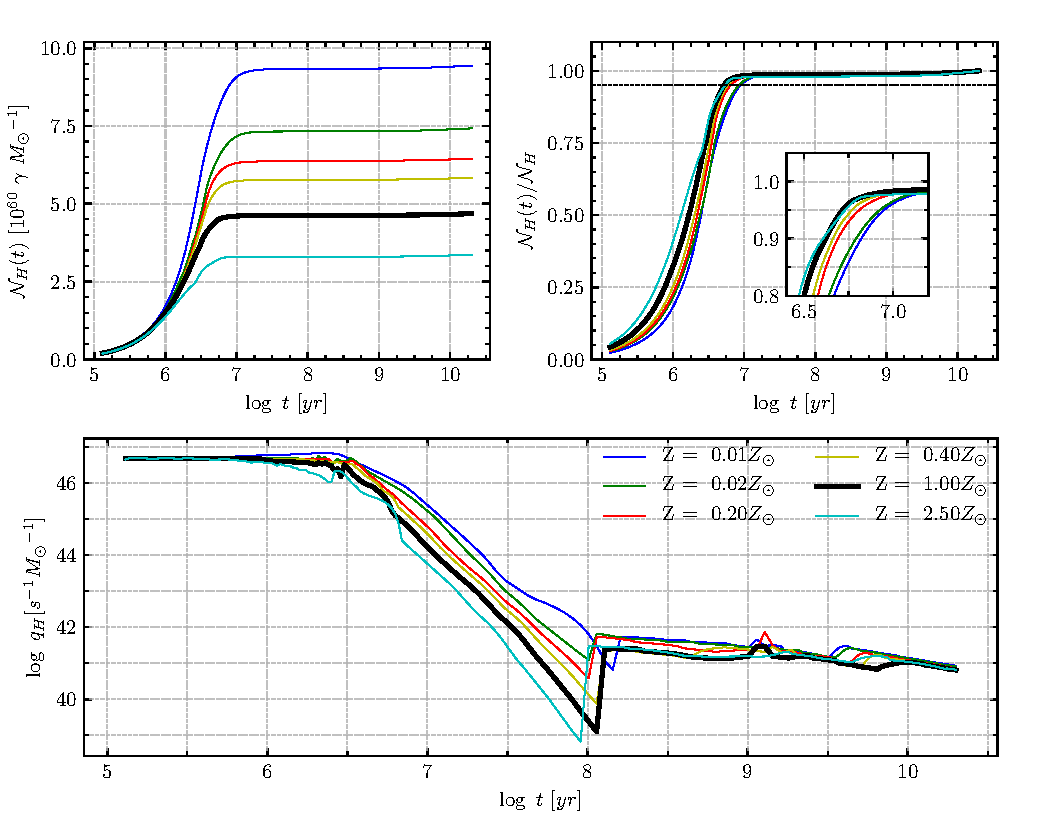
\includegraphics[width=\textwidth]{Nh_logt_metBase_Padova1994_chab.pdf}
    \caption{\emph{Upper left panel}: The time-evolution of the number of the photons ($\mathcal{N}_H$) for six metallicities (from 0.01 $Z_\odot$ to 2.5 $Z_\odot$) that compose our SSP models. The solar metallicity is drawn as a thick black line. \emph{Upper right panel}: The same from \emph{upper left panel} but normalized by the total value of $\mathcal{N}_H$. The black dashed line shows 95\% of the total $\mathcal{N}_H$. A zoom is also provided for a better view of the region around 10 Myr. \emph{Bottom panel}: Evolution of the H-ionizing photon rate per unit formed mass also for the same six metalicities. For this version of figure we use 'Padova 1994' stellar tracks \citep{Bertelli.etal.1994} with a Chabrier extinction law.}
    \label{fig:Nh_qh_Padova1994_chab}
\end{figure*}

\begin{figure*}
    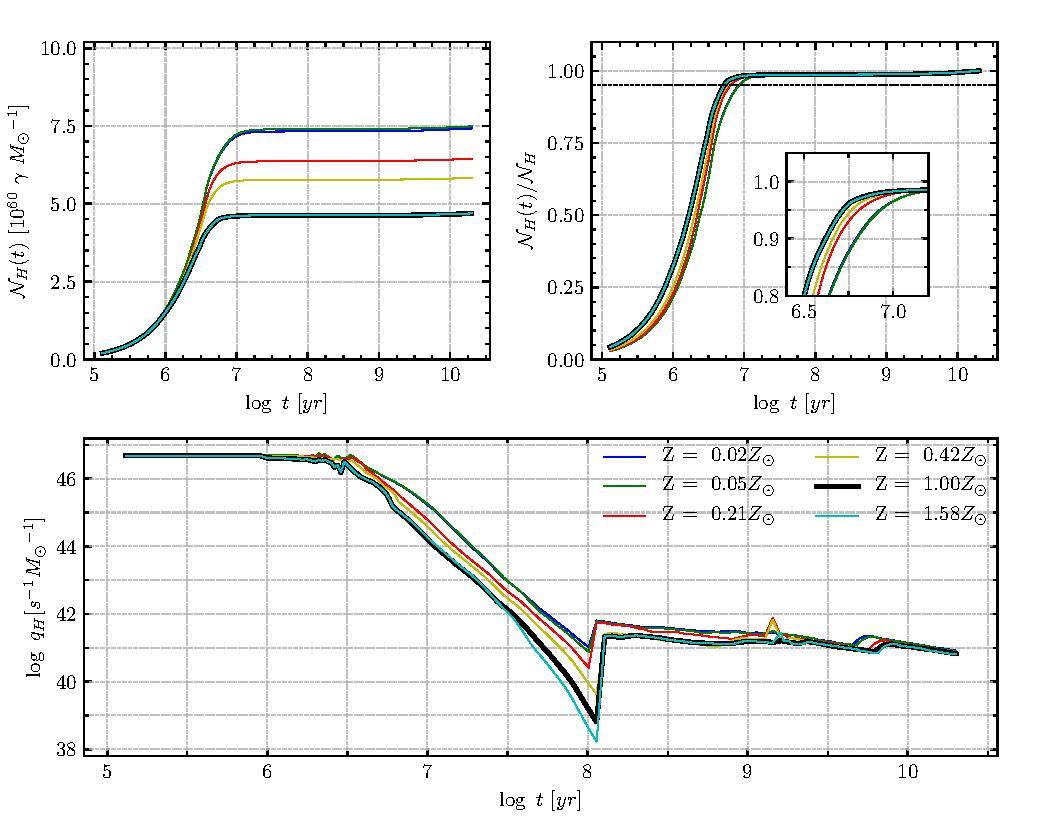
\includegraphics[width=\textwidth]{Nh_logt_metBase_Padova2000_chab.pdf}
    \caption{The same as Fig. \ref{fig:Nh_qh_Padova1994_chab} but with stellar tracks from \citep{Girardi.etal.2000a} (a.k.a. Padova 2000) and also a \citet{Chabrier.2003a} IMF. The metallicities for this configuration goes from 0.02 $Z_\odot$ to 1.58 $Z_\odot$.}
    \label{fig:Nh_qh_Padova2000_chab}
\end{figure*}

\begin{figure*}
    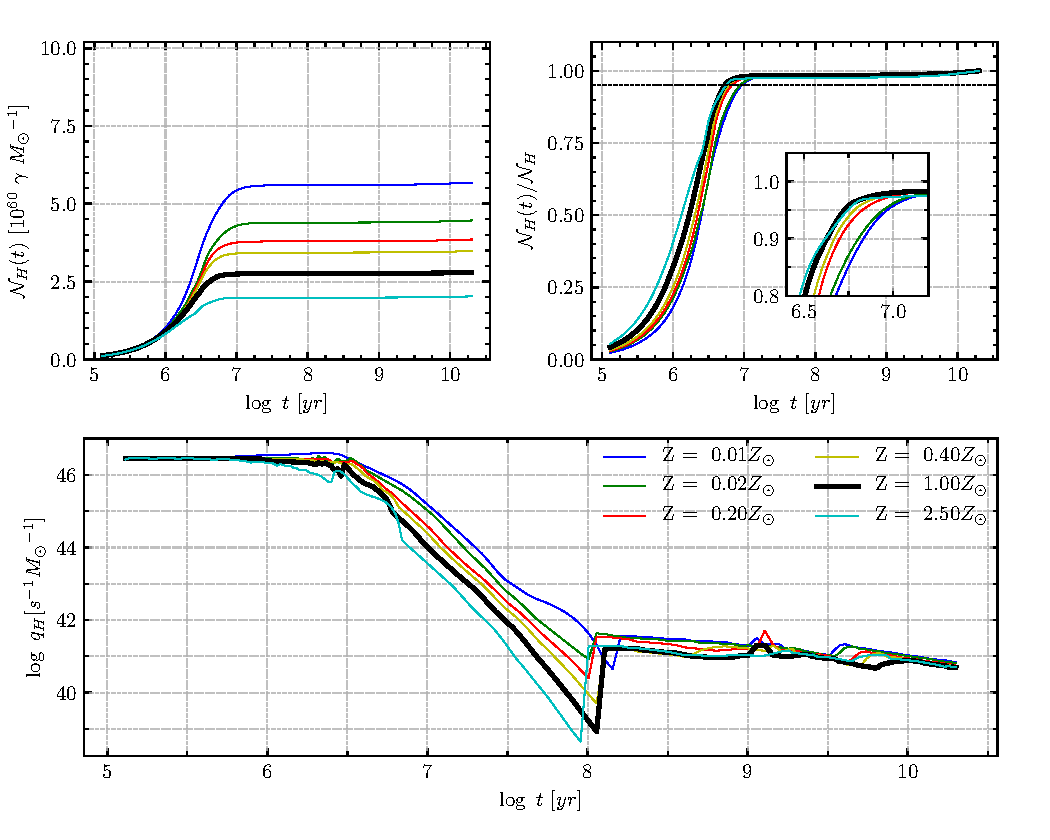
\includegraphics[width=\textwidth]{Nh_logt_metBase_Padova1994_salp.pdf}
    \caption{The same as Fig. \ref{fig:Nh_qh_Padova1994_chab} but with a \citet{Salpeter.1955a} IMF.}
    \label{fig:Nh_qh_Padova1994_salp}
\end{figure*}

\begin{figure*}
    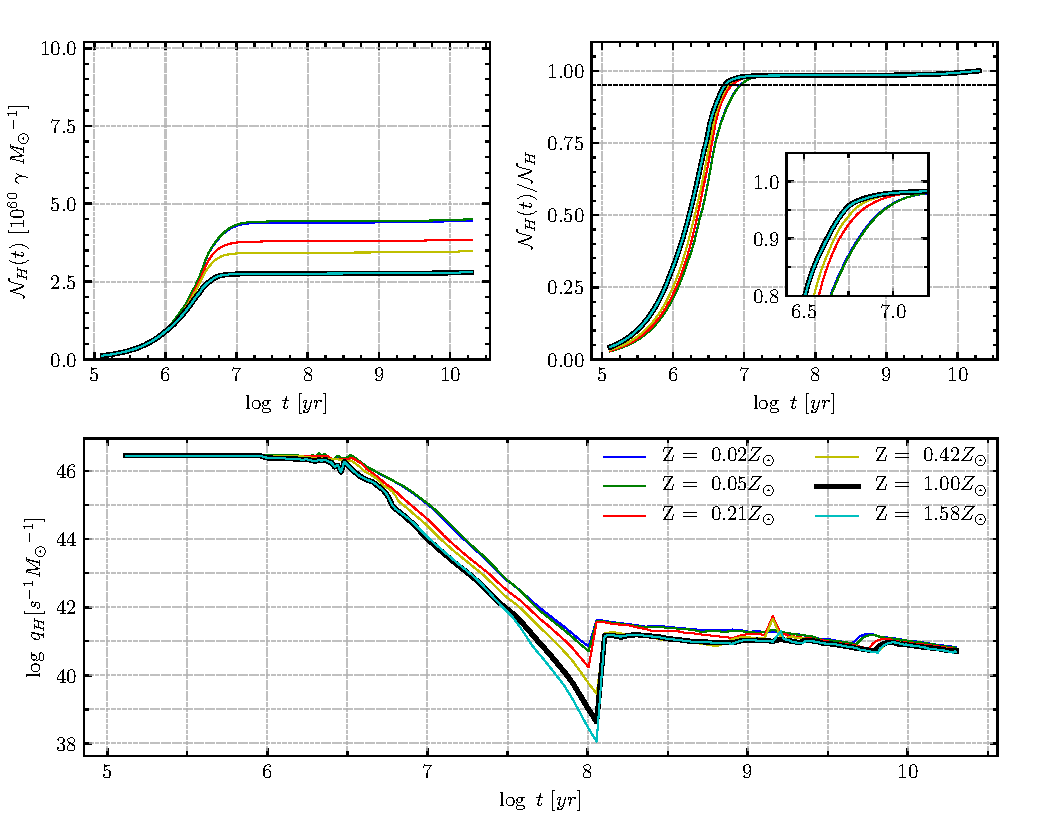
\includegraphics[width=\textwidth]{Nh_logt_metBase_Padova2000_salp.pdf}
    \caption{The same as Fig. \ref{fig:Nh_qh_Padova2000_chab} but with a \citet{Salpeter.1955a} IMF.}
    \label{fig:Nh_qh_Padova2000_salp}
\end{figure*}

Using \citet{BC03a} SSP models we can see the evolution of $\mathcal{N}_H$ in time in the Figs. \ref{fig:Nh_qh_Padova1994_chab}, \ref{fig:Nh_qh_Padova2000_chab}, \ref{fig:Nh_qh_Padova1994_salp} and \ref{fig:Nh_qh_Padova2000_salp}. This figure shows us the evolution of $\mathcal{N}_H$ in time in absolute values (left-upper panel) and in relatively the total $\mathcal{N}_H$ (right-upper panel). In \citet[Fig. 2b]{CF.etal.2011} we can see the time evolution of $q_H$ over all ages and metalicities\footnote{In that study the \href{http://starlight.ufsc.br}{SEAGal/\STARLIGHT} group used 'Padova 1994' \citep{Bertelli.etal.1994} stellar tracks with an IMF from \citet{Chabrier.2003a}}. The same plot is reproduced here at the bottom panel of Fig. \ref{fig:Nh_qh_Padova1994_chab}. It's easy to twig that the number of H-ionizing photons rapidly converges to its maximum close to $t=10$ Myr. For an SFR which is constant over that time-scale ($\psi(t) \rightarrow \psi$) the Eq. \ref{eq:QH} converges to
\begin{equation}
	\mathrm{Q}_H = \psi\ \mathcal{N}_H(t=10\textrm{Myr, IMF, Z}{}_\star).
	\label{eq:QH_converge}
\end{equation}
\noindent Replacing Eq. \ref{eq:QH_converge} in Eq. \ref{eq:LHa_recomb_theory}, we are now able to write:
\begin{equation}
	\psi_{\Ha} = \frac{2.206}{\mathcal{N}_H\ h \nu_{\Ha}} \times \LHalpha
	\label{eq:SFR_theoric}
\end{equation}
\noindent This method gives us a recent SFR. Recent because we use the value of $N_H$ at $t=10$ Myr. For the last step, solving Eq. \ref{eq:SFR_theoric} we found the value for k in Eq. \ref{eq:SFRHa} ($\psi \equiv \mathrm{SFR}$) for solar metallicity, Padova (2000) stellar tracks and an IMF from Salpeter (thick black line in Fig. \ref{fig:Nh_qh_Padova2000_salp}):
\begin{equation}
	\mathrm{SFR}_{\Ha} [\mathrm{M}_\odot\ \mathrm{yr}^{-1}] = 3.21\left(\frac{\LHalpha}{10^8\mathrm{L}_\odot}\right) = 8.38 \times 10^{-42}\ \LHalpha\  [\mathrm{ergs}\ \mathrm{s}^{-1}]
	\label{eq:SFRNeb}
\end{equation}
In Table \ref{tab:k} we show the value of k for each set of models and metallicity, the fraction of ionizing photons at $t=10$ Myr and the age where the fraction of ionizing photons is 95, 98 and 99 per cent. Fig. \ref{fig:k} brings the distribution of k in function of metallicity for all models. For the IMF of \citet{Salpeter.1955a}, the values of k changes in metallicity from a factor of $\sim$ 1.5 for Padova2000 to $\sim$ 3 for Padova1999 configuration. Changing to a \citet{Chabrier.2003a} IMF, the values of k varies in a factor of $\sim$ 2 for Padova2000 for almost 10 for the Padova1994 isochrones. We have to take in account that for the Padova2000 models, the metallicity range from 0.02 Z$_\odot$ to $\sim$ 1.6 Z$_\odot$, when Padova1994 models goes from 0.005 Z$_\odot$ to 2.5 Z$_\odot$. The \citet{Kennicutt.1998a} calibration for solar metallicity (7.9 $\times$ 10$^{-42}$ ergs s$^{-1}$) was calculated with other SSP models and with a \citet{Salpeter.1955a} IMF. 

\begin{table}
    \centering
    \resizebox{\columnwidth}{!} {
    \begin{threeparttable}
        \caption{List of values of k for each model and metallicity. Together we add the fraction of ionizing photons at $t=10$ Myr, $\mathcal{N}_H(10Myr)/\mathcal{N}_H^{\mathrm{tot}})$ and the ages where the fraction of ionizing photons is 95, $t_{95}$, 98, $t_{98}$ and 99 per cent, $t_{99}$.}
        \begin{tabular}{l|c|c|c|c|c|c|c}
            \hline
            Set of models & Z & k [M$_\odot$ yr$^{-1}$] & k [10$^{-42}$ ergs s$^{-1}$] & $\mathcal{N}_H(10Myr)/\mathcal{N}_H^{\mathrm{tot}}$ & $t_{95}$ [Myr] & $t_{98}$ [Myr] & $t_{99}$ [Gyr] \\
            \hline
            \hline
            Padova1994.chab & 0.0001 & 0.97 & 2.54 & 0.9615 & 8.71 & 13.80 & 0.81 \\
            Padova1994.chab & 0.0004 & 1.23 & 3.21 & 0.9657 & 8.32 & 13.18 & 2.75 \\
            Padova1994.chab & 0.0040 & 1.40 & 3.65 & 0.9783 & 6.31 & 10.47 & 2.20 \\
            Padova1994.chab & 0.0080 & 1.54 & 4.02 & 0.9813 & 5.75 & 9.12 & 2.20 \\
            Padova1994.chab & 0.0200 & 1.91 & 5.00 & 0.9834 & 5.01 & 7.94 & 2.75 \\
            Padova1994.chab & 0.0500 & 2.68 & 7.00 & 0.9775 & 5.25 & 508.80 & 7.75 \\
            Padova1994.salp & 0.0001 & 1.62 & 4.24 & 0.9574 & 9.12 & 15.85 & 3.25 \\
            Padova1994.salp & 0.0004 & 2.05 & 5.36 & 0.9616 & 8.71 & 15.85 & 5.00 \\
            Padova1994.salp & 0.0040 & 2.34 & 6.13 & 0.9749 & 6.61 & 12.59 & 5.00 \\
            Padova1994.salp & 0.0080 & 2.59 & 6.76 & 0.9783 & 6.03 & 10.47 & 5.25 \\
            Padova1994.salp & 0.0200 & 3.21 & 8.39 & 0.9806 & 5.25 & 9.55 & 5.50 \\
            Padova1994.salp & 0.0500 & 4.47 & 11.68 & 0.9734 & 5.50 & 2600.00 & 9.50 \\
            Padova2000.chab & 0.0004 & 1.23 & 3.21 & 0.9660 & 8.32 & 13.18 & 2.40 \\
            Padova2000.chab & 0.0010 & 1.22 & 3.18 & 0.9652 & 8.32 & 13.18 & 1.90 \\
            Padova2000.chab & 0.0040 & 1.40 & 3.65 & 0.9786 & 6.31 & 10.47 & 1.90 \\
            Padova2000.chab & 0.0080 & 1.54 & 4.02 & 0.9818 & 5.75 & 9.12 & 1.80 \\
            Padova2000.chab & 0.0190 & 1.91 & 5.00 & 0.9830 & 5.01 & 7.94 & 3.75 \\
            Padova2000.chab & 0.0300 & 1.91 & 4.99 & 0.9829 & 5.01 & 8.32 & 3.25 \\
            Padova2000.salp & 0.0004 & 2.05 & 5.36 & 0.9618 & 8.71 & 15.85 & 5.50 \\
            Padova2000.salp & 0.0010 & 2.03 & 5.32 & 0.9612 & 8.71 & 15.14 & 5.00 \\
            Padova2000.salp & 0.0040 & 2.34 & 6.13 & 0.9753 & 6.61 & 12.02 & 4.75 \\
            Padova2000.salp & 0.0080 & 2.59 & 6.76 & 0.9788 & 5.75 & 10.47 & 4.25 \\
            Padova2000.salp & 0.0190 & 3.21 & 8.39 & 0.9800 & 5.25 & 9.55 & 6.75 \\
            Padova2000.salp & 0.0300 & 3.21 & 8.38 & 0.9800 & 5.25 & 9.55 & 6.25 \\
            \hline   
        \end{tabular}
    \end{threeparttable}
    }
    \label{tab:k}
\end{table}

\begin{figure*}
    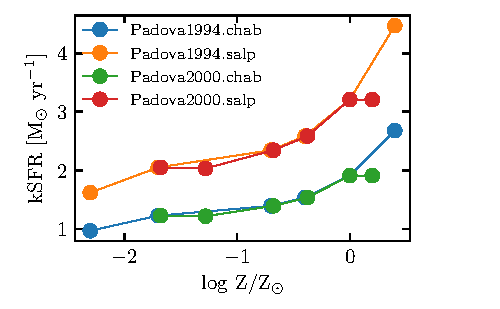
\includegraphics[width=\textwidth]{logZ_kSFR_bases.pdf}
    \caption{}
    \label{fig:k}
\end{figure*}


\bibliographystyle{mnras}
\bibliography{bibliography}

% \newpage
% \appendix

% \section{The creation rate of \Ha photons}
% \label{app:Ha}

% Consider a volume element $\Delta V$ in an \Hii\ region. The number of $p + e \rightarrow {\rm H}^0$ recombinations per unit time is $n_p n_e \alpha_B({\rm H}^0) \Delta V$, where $n_e$ and $n_p$ are the proton and electron densities, and $\alpha_B({\rm H}^0)$ is the case B total recombination coefficient of H. From Table 2.7 in \citet{Osterbrock.Ferland.2006a} $\alpha_B({\rm H}^0) = 2.59\times10^{-13}$ recombinations$\,\times\,$cm$^3\,$s$^{-1}$ (for a temperature of 10000 K). During the recombination cascade some of these re-married electrons will go through  $n = 3 \rightarrow 2$ transitions, producing \Ha. Let $\alpha_{\Ha}^{eff}({\rm H}^0)$ be the coefficient which counts only these recombinations. $\alpha_{\Ha}^{eff}({\rm H}^0)$ is not explicitly given in Osterbrock \& Ferland's book, but they do provide (in Table 4.7) the coefficient for \Hb, $\alpha_{\Hb}^{eff}({\rm H}^0) = 3.03\times10^{-14}$, as well as the ratio of volume emissivities, the famous $j_{\Ha}/j_{\Hb} = 2.87$. Using
% $$
% \frac{ \alpha_{\Ha}^{eff}({\rm H}^0) }{ \alpha_{\Hb}^{eff}({\rm H}^0) } = \frac{ j_{\Ha} / h\nu_{\Ha} }{ j_{\Hb} / h\nu_{\Hb} }
% $$
% \noident (where the ratio of photon energies appears because $j$ measures energy while $\alpha$ measures a number of recombinations), we finally 
% obtain $\alpha_{\Ha}^{eff}({\rm H}^0) = 1.17\times10^{-13} \,$cm$^3\,$s$^{-1}$ , or $0.453 \times \alpha_B({\rm H}^0)$. In other words, one out of every $1/0.453 = 2.206$ recombinations produces an \Ha photon. Since in equilibrium each photoionization is balanced by a recombination, and as long as no $h\nu > 13.6$ eV radiation escapes the nebula, we can also say that one out of every 2.206 ionizing photons produces on \Ha photon.

\end{document}